\section{Design}\label{sec:design}

\begin{figure*}[t]
    \centering
    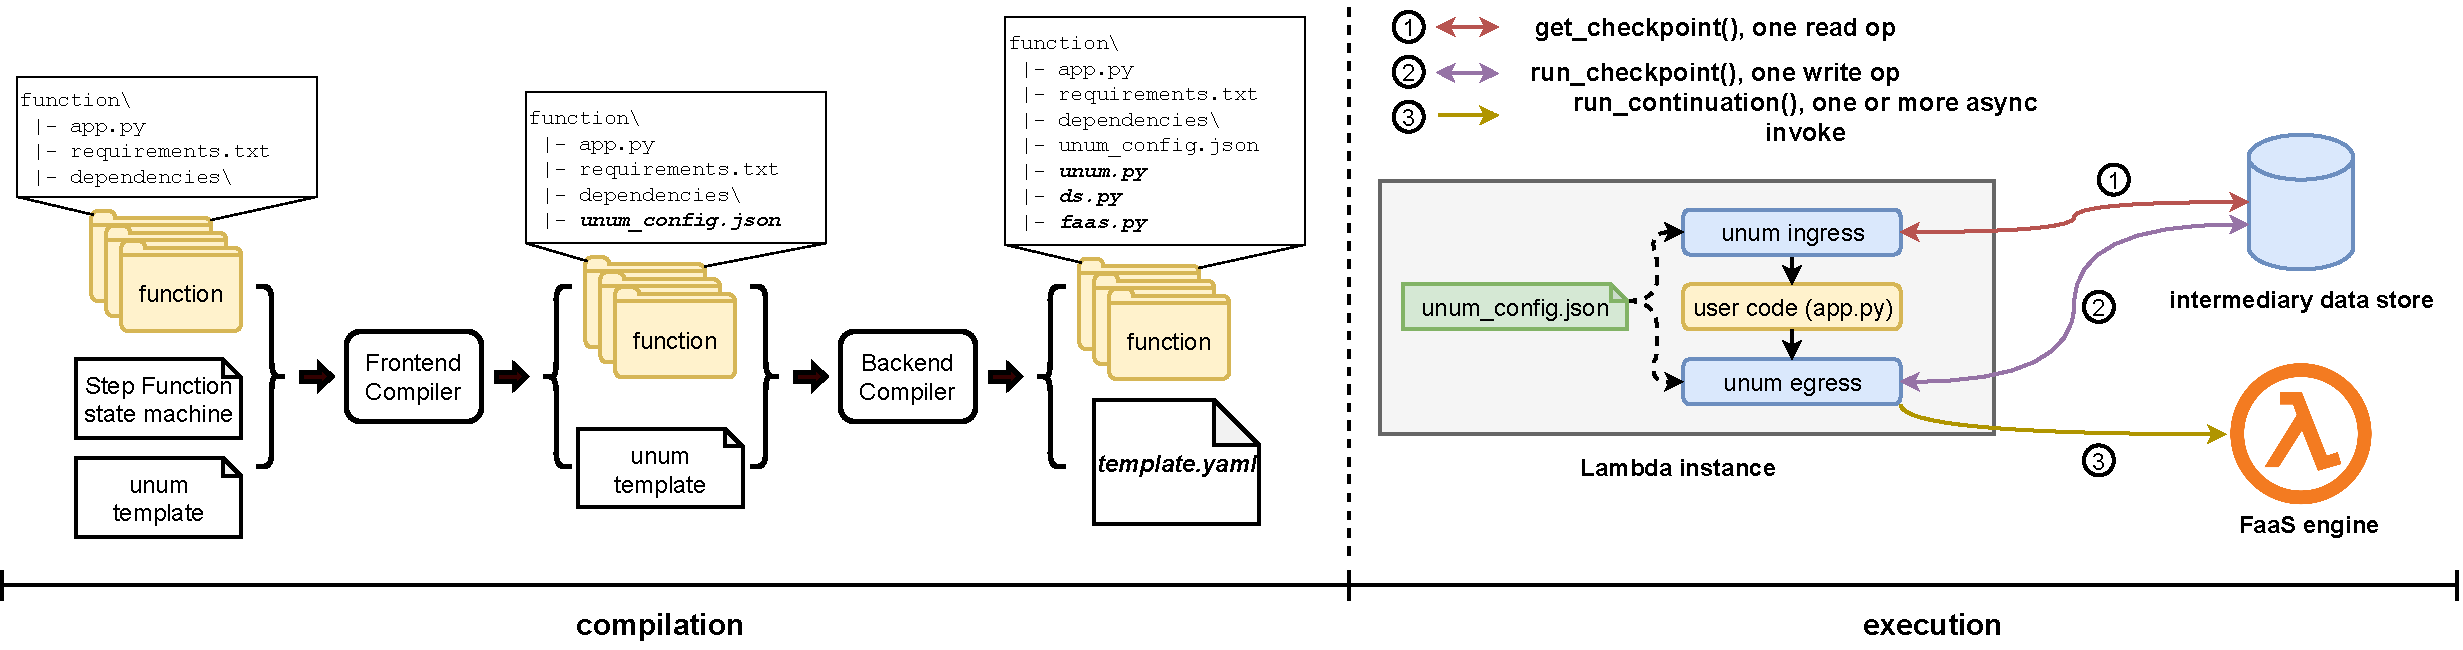
\includegraphics[width=\textwidth]{figures/unum-arch.pdf}
    \caption{\name{}'s architecture}
    \label{fig:arch}
\end{figure*}

\begin{figure}[]
    \begin{minted}[
    frame=single,
    linenos,
    fontsize=\footnotesize
  ]{yaml}
Globals:
  ApplicationName: unum-iot-chain
  UnumIntermediaryDataStoreType: dynamodb
  UnumIntermediaryDataStoreName: iot-intermediary
  Checkpoint: true
  Debug: false
Functions:
  Aggregator:
    Properties:
      CodeUri: aggregator/
      Runtime: python3.8
      Start: true
  HvacController:
    Properties:
      CodeUri: hvac_controller/
      Runtime: python3.8
      Policies:
        - AmazonSQSFullAccess
  \end{minted}
    \caption{The unum template for an IoT HVAC controller
    application. It lists all resources of the workflow (Two functions:
    \texttt{Aggregator} and \texttt{HvacController}. A DynamoDB table
    \texttt{iot-intermediary} used as the intermediary data store) and
    specifies workflow-wide options such as checkpoint, debug and
    application name.}
    \label{fig:iot-unum-template}
\end{figure}


\begin{figure}[]
    \begin{minted}[
    frame=single,
    linenos,
    fontsize=\footnotesize
  ]{json}
{
  "StartAt": "Aggregator",
  "States": {
    "Aggregator": {
      "Type": "Task",
      "Resource": "Aggregator",
      "Next": "HvacController"
    },
    "HvacController": {
      "Type": "Task",
      "Resource": "HvacController",
      "End": true
    }
  }
}
    \end{minted}
    \caption{A Step Functions state machine for an IoT HVAC controller
    application. The workflow is a chain of two functions \texttt{Aggregator}
    and \texttt{HvacController}. When \texttt{Aggregator},
    \texttt{HvacController} should be invoked with \texttt{Aggregator}'s
    result. Note that normally the \texttt{"Resource"} fields are the deployed
    Lambda's ARN. Here they are function names defined in the unum template
    (see Figure~\ref{fig:iot-unum-template})}
    \label{fig:iot-sf}
\end{figure}

A key feature in \name{}'s approach is that it is designed as a runtime on top
of the serverless abstraction without requiring any supplemental services
added to current infrastructures. Workflows built with \name{} can execute in
any environment that has a FaaS engine with an asynchronous invocation API and
a named data store that supports strongly consistent reads. Both are readily
available on all existing serverless platforms.

Architecturally, \name{} eliminates the need for any specialized, hosted
processes that execute workflows, manage system states or broker
inter-function communication. FaaS functions are the only compute entity in
\name{} that runs code. They execute both user code and the \name{} runtime. The
\name{} runtime directly invokes the next function in the workflow after user
code completes and leverages a checkpointing mechanism to ensure strong
execution guarantees.

We continue this section by first giving an overview of unum's architecture
and outlining the serverless abstractions and services that \name{} builds
upon (Sec.~\ref{sec:sys-req}). We then describe the programming interface that
\name{} supports. Next, we discuss the \name{} IR, \name{}'s internal
representation of workflows, which expresses serverless workflows using
continuations. Finally, we describe \name{}'s runtime wrapper and execution
guarantees.%, how it interposes on user code, what runtime metadata it manages and how it
% leverage checkpointing to provide a strong execution guarantee that we term
% \emph{at-least-once execution with exactly-one result}.

\subsection{Overview}

Figure~\ref{fig:arch} shows \name{}'s high-level architecture. At
compile-time, a frontend compiler transforms workflows written for existing
systems (e.g., an AWS Step Functions state machine that orchestrates Lambdas)
into a continuation-based, platform-independent intermediary representation
(Sec.~\ref{sec:unum-ir}). In practice, the IR is a set of configuration files
(\texttt{unum\_config.json}), one for each function in the workflow, written
in the \name{} configuration language (Sec.~\ref{sec:design-config-lang}).

Then a backend compiler compiles the IR into platform-specific packages that
are executable in a particular target environment (e.g., AWS Lambda with
DynamoDB as the data store). Deploying the packages will create a set of FaaS
functions (e.g., Lambdas) and an intermediary data store (e.g., a DynamoDB
table or S3 bucket).

A workflow is invoked by triggering the entry function. Each unum workflow has
one and only one entry function.

At execution time, each function runs both the user code and the unum runtime.
The unum runtime manages the function's checkpoint and invokes the
continuation asynchronously after user code completes. unum uses checkpoints
to provide strong execution guarantee. Every function invocation in unum is
assigned a unique name and the runtime uses the name for the instance's
checkpoint in the data store.

\subsection{System Requirements}

\name{} utilizes two services that are readily available on all existing
serverless platforms:

\begin{enumerate}

	\item A Function-as-a-Service engine that supports an
	\emph{asynchronous invocation API}.

	\item A shared data store that supports creating and reading items by
	 their unique names.

\end{enumerate}

\subsubsection{FaaS engine with asynchronous invocation}

Support for asynchronous invocation is universal across all major FaaS
engines, including AWS Lambda~\cite{aws-lambda-async-invoke}, Azure
Functions~\cite{azure-functions-async-invoke}, Google Cloud
Functions~\cite{google-cloud-functions-async-invoke}, and popular open-source
options such as OpenWhisk~\cite{openwhisk-async-invoke} and
OpenFaaS~\cite{openfaas-async-invoke}.

\name{} chooses asynchronous invocation because functions in \name{} directly invoke
their immediate downstream functions and asychronous invocation avoids
timeouts, and double billing. If only synchronous invocation is available, a
function has to idly wait for all of its downstream functions, immediate or
not, to complete, risking function timeouts and incurring double billing.

\paragraph{At-least-once invocation}

FaaS engines normally only guarantee at-least-once invocation of
asynchronously triggered
functions~\cite{google-cloud-functions-exec-guarantee,
aws-lambda-async-invoke, azure-functions-exec-guarantee}. A single invocation
might result in the FaaS engine running the same function more than once. Such
duplicate invocations are especially problematic when the function is
non-deterministic (i.e., given the same input, the function might produce
different output across runs) and all serverless providers simply urge
developers to write deterministic functions to avoid incorrect behavior.

From a workflow system's perspective, it has a few options to work with an
at-least-once FaaS engine: (1). it can equire all functions to be
deterministic (2). make sure functions are invoked exactly-once (3). ensure
that even if a non-deterministic function executes more than once, only one of
the results is taken as the final result and propagated to the rest of the
workflow.

\name{} takes the third approach as the first is restrictive and the second is
unattainable. \name{} uses a checkpointing mechanism to make sure only the
execution that finishes first is taken as the final result and propagated
downstream. Duplicates are simply discarded. We discuss the details in
Sec.~\ref{sec:design-runtime}.

\subsubsection{Named data store}

Functions in \name{} workflows use a named data store to store checkpoints and
other intermediary data (Sec.~\ref{sec:design-runtime}) during execution. The
data store needs to support creating and later retrieving objects with unique
names.

There is a wide variety of data store services that can support \name{}
workflows, including object storage (e.g., Amazon S3, AZure Blob Storage),
NoSQL databases (e.g., DynamoDB, Cosmos DB) and key-value stores (e.g.,
Redis).

Nearly all of the storage services above have a "serverless" option that
requires no explicit provisioning and users only pay for what they use.

\paragraph{Consistency Requirements}

\name{} requires the data store to be strongly consistent.

Strongly consistent reads (read that return the most up-to-date data,
reflecting all prior writes that were successful) are important for the
correctness of aggregations (e.g., fan-in), because it prevents the
possibility where all upstream functions have completed and written their
checkpoint but none of them sees that all have completed and thus never invoke
the fan-in function.

Note that strong consistency alone is not enough for correct execution of
aggregation patterns because multiple functions might detect that all fan-out
branches have completed and thus invoking the fan-in functions more than once.
\name{} runtime contains additional synchronization logic to make sure the fan-in
function is only invoked once. We discuss the details in
Sec.~\ref{sec:design-runtime}


\subsection{Programming Interface}

\name{} does not introduce a new programming interface for building serverless
workflows. Developers can use familiar frontend languages from existing
systems, such as the Amazon State Language for AWS Step Functions.

Moreover, \name{} lets developers write component functions in
workflows exactly the same way as they would for regular functions. In fact,
orchestration-related logic are entirely transparent from user functions'
perspective. There is no additional libraries that user code needs to import
or use.

Figure~\ref{fig:arch} gives an example of using Step Functions state machine
to define the workflow that orchestrates functions in Python. Each
function is defined in its own directory with the exact same content as you
would have for regular functions that are not part of any workflow.

The \emph{unum template} is a YAML file that lists all the resources in the
workflow and specifies workflow-wide configurations.
Figure~\ref{fig:iot-unum-template} gives an example of an IoT HVAC controller
application's template.

The frontend compiler transforms the workflow definition to a
continuation-based, platform-independent intermediary representation (IR)
which we discuss in the next section.



\subsection{\name{} IR}

The \name{} intermediary representation expresses FaaS workflows using
continuations. A continuation defines (1). which function(s) to invoke (2).
what input to invoke it with.

Every function in a unum workflow has 0, 1 or more continuations. After
running user code, the unum runtime invokes the continuation with the user
code's result as the input. The set of continuations from all functions form
the complete workflow.

The purpose of the continuation-based IR is to distribute workflows'
orchestration logic to individual component functions so that it can execute
without a centralized orchestrator. In an orchestrator-based workflow system,
functions will need to call back to the orchestrator service to signal
completion and it is the orchestrator who will then invoke the next function.

In contrast, unum assigns each function a set of continuations at
compile-time. After user code completes, each function directly invokes its
continuations asynchronously, without involving any supplemental services.

\subsubsection{\name{} configuration language}

In practice, the \name{} IR is a set of configuration files, one for each
function in the workflow, written in the \name{} configuration language
(\ref{sec:design-config-lang}). The configuration language provides constructs
to define continuations and modify runtime metadata.

Figure~\ref{fig:iot-sf} shows a Step Functions state machine for an IoT HVAC
controller workflow which is a chain of two functions. Figure~\ref{fig:iot-ir}
shows the generated IR in the form of two \texttt{unum\_config.json} files.

\begin{enumerate}

	\item The meaning and effects of "InputType": Scalar, Map, Fan-in

	\item The meaning and effects of "Conditional": branch

	\item "Start"

	\item "Next Payload Modifiers": the interface to manipulate runtime metadata (\$size, \$0)

\end{enumerate}


\subsection{Runtime}


\subsubsection{Payload structure and metadata}


\subsubsection{Checkpoints?}


check checkpoint existence before running user function

run user function or read from existing checkpoint

write checkpoint or pass

run continuation

checkpoints are used both for guaranting execution correctness and for
aggregation patterns such as fan-in.


\subsection{Fault tolerance and execution guarantee}

